%Microsoft Windows family (namely 2003-current Server, 3.1.1-current), Linux (namely Ubuntu, Mint Cinnamon, and Kali), Android and iOS

\documentclass[tikz,border=2mm]{standalone}

\begin{document}
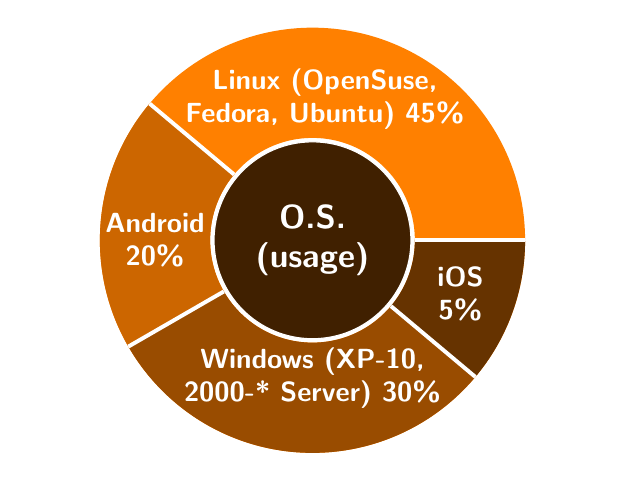
\begin{tikzpicture}[font=\sffamily\bfseries\large, 
     text=white, 
     border/.style={line width=14mm}]
\foreach \angle/\col [remember=\angle as \last (initially 0)] in 
    {360/orange!100!black, 320/orange!40!black, 210/orange!60!black, 140/orange!80!black, 140/orange!80!black}{    
		\draw[\col, border] (\last:2cm) 
             arc[start angle=\last, end angle=\angle, radius=2cm];
		\draw[white, line width=0.5mm] (\last:1.3)--++(\last:1.4);
}
\node[text width=1.5cm, align=center, font=\sffamily\bfseries\large, draw, circle, minimum width=2.5cm, white, fill=orange!25!black] {O.S. (usage)};
\node[text width=6.5cm, align=center, font=\sffamily\bfseries\normalsize] at (85:1.80cm) 
	{Linux (OpenSuse, \\ Fedora, Ubuntu) 45\% };
\node[text width=3.0cm, align=center, font=\sffamily\bfseries\normalsize] at (180:2cm) 
    {Android \\ 20\%};
\node[text width=6.5cm, align=center, font=\sffamily\bfseries\normalsize] at (270:1.75cm) 
    {Windows (XP-10, \\ 2000-* Server) 30\%};  
\node[text width=1.1cm, align=center, font=\sffamily\bfseries\normalsize] at (340:2cm) {iOS 5\%};
\end{tikzpicture}
\end{document}
